The numerical framework in this project is novel as the existing models are quasi-static such that the velocity and acceleration are assumed to be $0$ in the momentum equation, therefore the left-hand side of Equation \ref{eq:momentum} becomes $\bold{0}$. Although this assumption is reasonable because the solid growth happens very slowly, it also fails to reflect the fact that the growth is immersed in fluid environment and the solid deformation is constantly disturbed by fluid flow. In our model, a disturbance will be given as the initial velocity of the fluid field, which will enforce a non-zero essential boundary condition on the solid tissue. 

\subsubsection{Fluid governing equations with mass flux}
Because of the mass transfer at the fluid-solid boundary, the mass equation needs to be modified. Recall the mass conservation of incompressible fluid states that the mass rate per unit volume is $0$, considering the mass flux, it is rewritten as:
\begin{equation}
\rho \nabla \cdot \bv = \nabla \cdot \bold{r}
\end{equation}
%\begin{equation}
%\rho \frac{D\bv}{Dt} = -\nabla p + \mu \nabla^2 \bv
%\end{equation}
where $\bold{r}$ is the mass flux in the current configuration. 

Let us also exam the momentum equation. In our IFEM formulation, the fluid mesh is fixed. The existence of the solid is detected by the ``artificial fluid". As the solid increases in volume, the artificial fluid will also increase in volume, which automatically takes care of the real fluid momentum on its own. Therefore, the momentum equation remains unchanged.

\subsubsection{Implementation}
Two improvements proposed are the mechanical stimulus from the fluid and the mass transfer from the fluid to the solid. Towards these ends, the overall framework must appropriately address these issues: (1) through the coupling of fluid and solid simulation, correctly identifying the mechanical stimuli applied to the solid growth, including both pressure and shear stress; (2) proposing reasonable assumptions on the mass flux, which is another essential impact on the growth process.

Figure \ref{fig:framework} represents the overall framework. It can be seen that the solid growth is fully coupled with fluid environment. Following our previous work in \cite{Zhang, Zhang3, Zhang16, Zhang17}, the fluid and solid are solved individually on different meshes. The interface velocity is distributed from the fluid to the solid and the volume force is distributed from the solid to the fluid. An initial disturbance is applied to the fluid, which is the only input to the coupled growth system except for the mass source.
\begin{figure}[H]
   \centering
   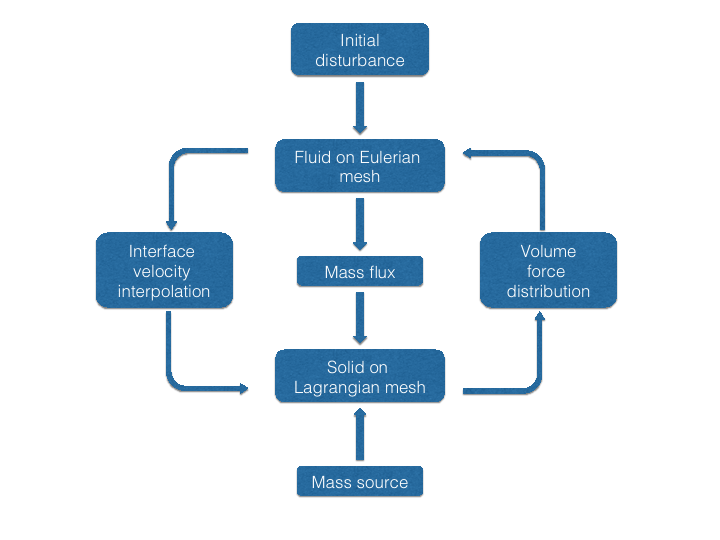
\includegraphics[width=.5\textwidth]{./figs/framework.png} % requires the graphicx package
   \caption{The numerical framework}
   \label{fig:framework}
\end{figure}





